In this section we describe our approach to the extraction of molecular surface and surfaces of inner cavities which we denote as surface features.
First we present the algorithms for the computation of molecular surfaces and cavities and then we show how we deal with special cases occurring within the surface construction.

%Extended CB Algorithm
\subsection{Surface computation}
\label{sec:ecb}
Our surface computation algorithm is based on the existing research that utilizes the GPU capabilities~\cite{krone2011parallel}.
In the former study, the SES is represented as three different sets of surface primitives -- spheres, tori, and spherical triangles, that are ray-casted to obtain opaque surface visualization. 
%While ray-casting spheres and tori, some sections of the final image will be later occluded by the spherical triangles.
\textcolor{red}{While ray-casting spheres and tori}, there are also produced pixels that are not visible in the final image, because of their occlusion by pixels on the surface (see Figure~\ref{fig:cb-krone}).
To enable transparent visualization of the surface, we extended the algorithm such that it employs following primitives:
%\textcolor{red}{JP: This needs to be explained: Therefore, to visualize contour surface representation using transparency}, we extended the algorithm so that it computes a SES represented with:
\begin{itemize}
	\item Spherical triangles.
  \item Toroidal patches -- a toroidal patch is delimited by two spherical triangles.
	\item Spherical patches -- a spherical patch is enclosed by edges of three or more toroidal patches.
\end{itemize}

\begin{figure}[htp]
  \centering
  \begin{subfigure}[t]{0.48\columnwidth}
    \centering
    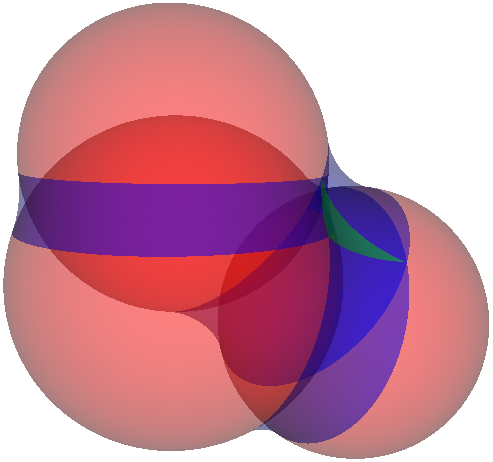
\includegraphics[width=1.5in]{image/cb-krone.png}
   % \caption{The original method \cite{krone2011parallel} rendered with transparency.}
		\label{fig:cb-krone}
  \end{subfigure}%
  ~
  \begin{subfigure}[t]{0.48\columnwidth}
    \centering
    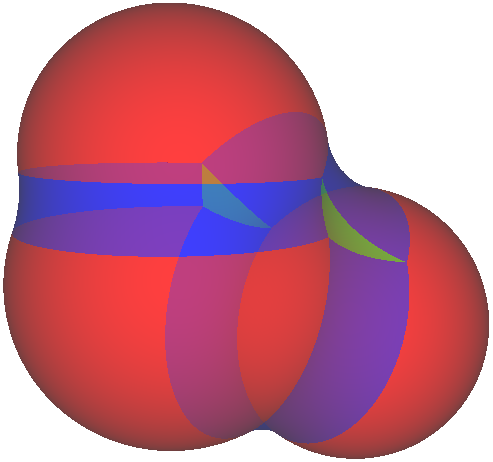
\includegraphics[width=1.5in]{image/cb-oit.png}
   % \caption{Our extended method.}
		\label{fig:cb-oit}
  \end{subfigure}
\caption{Comparison between the original method~\cite{krone2011parallel} rendered with transparency (left) and our extended method (right).
%The transparent SES of three atoms produced by the original parallel CB algorithm (a), and our extended algorithm (b). 
The original method renders parts of spheres (red) and tori (blue) that lie below the surface.
Our method produces only primitives that are part of the surface.
%More, our algorithm is also able to handle patches on a sphere that form different surfaces, i.e., the outer and one or more inner.
}
\end{figure}

In comparison with the previous solution our main contribution here lies in the computation of toroidal and spherical patches.
Using them we avoid the situation when the previous algorithm renders parts of tori and spheres which do not form the final surface (see Figure~\ref{fig:cb-oit}).

%Regarding tori, Kauker et al.~\cite{kauker2013rendering} proposed to ray-cast a toroidal patch using a torus and two clipping planes defined by its delimiting triangles.

%\begin{figure}[htp]
%  \centering
%  \begin{subfigure}[t]{0.55\columnwidth}
%    \centering
%    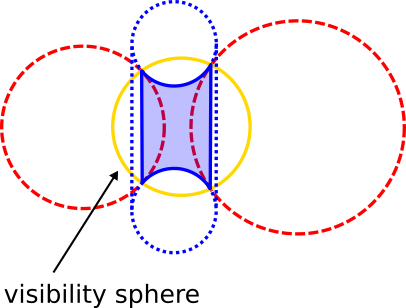
\includegraphics[width=1.7in]{image/torus-vs.png}
%    \caption{Clipping by \textit{visibility sphere}.}
%		\label{fig:torus-vs}
%  \end{subfigure}%
%  \quad
%  \begin{subfigure}[t]{0.4\columnwidth}
%    \centering
%    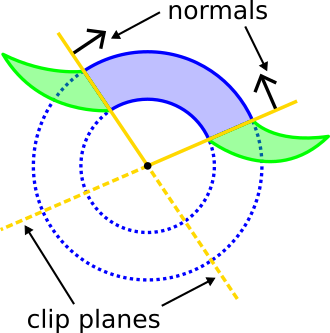
\includegraphics[width=1.3in]{image/torus-planes.png}
%    \caption{Clipping by planes defined by spherical triangles.}
%  \end{subfigure}
%\caption{Ray-tracing of a toroidal patch. The saddle part of the torus (a) is cut by so called \textit{visibility sphere}.
%A patch (b) is cut from the whole toroidal ring by clipping planes.}
%\end{figure}

%We employ his approach and modify the data structure that is used in the original algorithm to store spherical triangles in such a way that we are able to obtain all triangles incident to a torus.
%In this way, we ray-cast toroidal patches directly instead of tori.
%In order to get all neighboring triangles for a torus, we hash the triangles by three keys -- one for each torus which is connected to a triangle.
%For this, we implemented a simple hash table (see Figure~\ref{fig:hashing}) which is based on linear addressing scheme \cite{alcantara2011efficient}.

%\begin{figure}[htb]
%  \centering
%  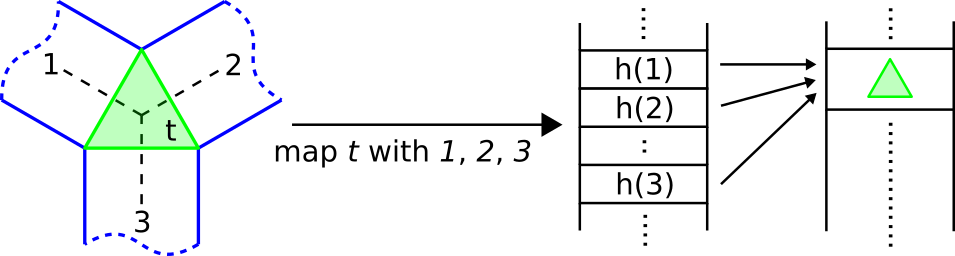
\includegraphics[width=3.3in]{image/hashing.png}
%  \caption{Our novel data structure for storing spherical triangles. Triangles $t_1$ and $t_2$ are stored linearly in an array and their incident torus $\tau$ is connected to them using a hash table.}
%	\label{fig:hashing}
%\end{figure}

To be able to compute toroidal patches, we introduce a novel data structure that enables to store and retrieve all spherical triangles incident to a torus (Fig.~\ref{fig:hashing41}). In order to get all neighboring triangles for a torus, we hash the triangles by three keys; i.e., one for each torus which is connected to a triangle.
For this purpose, we implemented a simple hash table, which is based on linear addressing scheme \cite{alcantara2011efficient}.
We find toroidal patches on a torus by retrieving all its neighboring triangles and sorting them relatively by their angular position around the torus.
We use the bubble sort algorithm for this sorting.
When sorted, the pairs of neighboring triangles define the toroidal patches and corresponding edges.
Additionally, we check whether the first two triangles form a visible patch.
If not, then the first triangle forms a visible patch with the last one and we rotate the sorted list of triangles by one item.
\begin{figure}[htb]
  \centering
  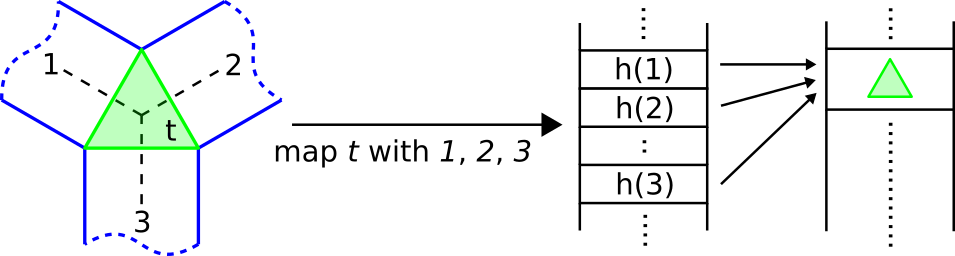
\includegraphics[width=3.3in]{image/hashing.png}
  \caption{An illustration of the data structure for storing spherical triangles. Triangles $t_1$ and $t_2$ are stored linearly in an array and their incident torus $\tau$ is connected to them using a hash table.}
	\label{fig:hashing41}
\end{figure}
This allows us, to ray-cast toroidal patches directly instead of tori.

As described, a spherical patch is bounded by toroidal patches (Fig~\ref{fig:graph}). We extended the surface computation algorithm by adding three new GPU kernels that compute the sets of toroidal patches forming the spherical patches (see Section~\ref{sec:graph}).
When visualizing the surface, each such set is used to ray-cast a spherical patch (see Section~\ref{sec:spherical-patches}).

%\begin{figure}[htb]
%  \centering
%  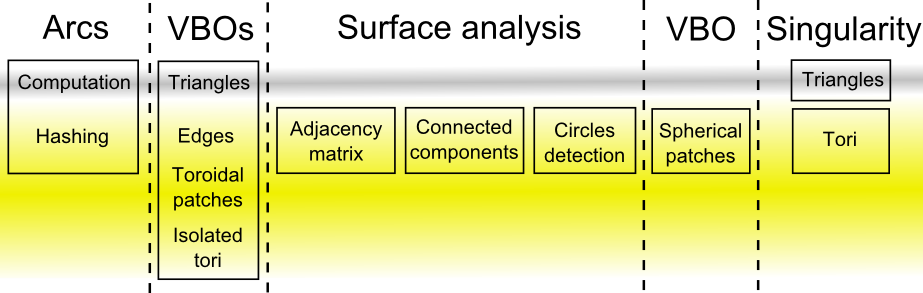
\includegraphics[width=3.3in]{image/kernels.png}
%  \caption{Overview of our extended algorithm.
%	The algorithm steps are ordered from the left to the right.
%	GPU kernels are marked with squares containing both original (grey) and our novel parts (yellow).}
%	\label{fig:kernels}
%\end{figure}

%Surface graph
\subsection{Cavity computation}
\label{sec:graph}
   
%\begin{itemize}
%  \item Idea: computed surfaces are continuous (closed) and graphs of their primitives form isolated components in the whole graph of all surface primitives
%  \item Modification of parallel CB of Krone et. al --- aaaa
%  \item Extension of parallel CB of Krone et. al --- 3 new kernels:
%	\begin{enumerate}
%	  \item Adjacency matrix is built (only 3 edges at each vertex)
%    \item Labeling of connected components (parallel BFS --- suboptimal)
%    \item Circles of edges for each spherical patch are computed
%  \end{enumerate}
%  \item Assign spheres with edges
%  \item Detect circles in edges --- bubble sort $O(n^2)$
%  \item Step 3 --- one sphere can form two or more surfaces
%  \item Rendering of spherical patches --- spherical polygons
%  \item Odd-even rule + point outside polygon
%  \item Special case: isolated tori
%\end{itemize}

The computed surface contains primitives of both the outer molecular surface and the surfaces of inner cavities.
%\footnote{\textcolor{red}{JP: This should be written in more friendly fashion and with clear defined terms. Terms to be explained: surface is continuitous (geometrical?, since $C^1$ continuous it is not), graphs (2D/3D, does it contain loops?), primitive, component}}
Kauker et al. \cite{kauker2013rendering} were in their study interested in visualizing only the outer surface.
%\footnote{\textcolor{red}{AJ: Maybe, this could be part of related work}}
Therefore, they called the inner parts of the surface as inner remains as it was source of occlusion.
However, the domain experts are often interested in the exploration of inner cavities because of their significant role in reactivity of the molecule.
%We think that for SES, the user might want to visualize cavities within the molecule and hence it is useful to let him decide on what to visualize.
So it is advantageous for the user to have the option to visualize both molecular surface and inner cavities and interactively change this decision.
It means that the cavities can be shown or hidden on demand.
%Contrary, for SAS, the cavities are visualized much smaller than in the case of SES and therefore visualizing them does not help assessing their shape or volume.
%The difference \textcolor{red}{stems from} the definitions of the surfaces.
%In the case of SAS, we therefore propose to clip the inner surfaces to enhance the visualization.

%The user might also want to hide cavities inside a SES to lower possible occlusion of other structures such as tunnels or cartoons.

\begin{figure}[htb]
  \centering
  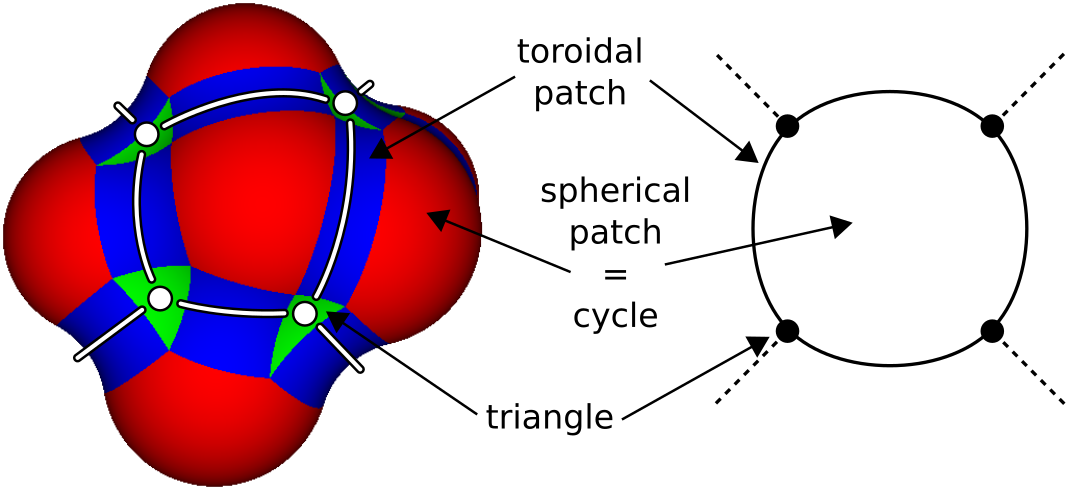
\includegraphics[width=3.3in]{image/graph.png}
  \caption{The surface graph.
	Triangles form vertices and toroidal patches form edges between them.
	Spherical patches are represented as cycles in the graph.}
	\label{fig:graph}
\end{figure}

The hiding of cavities is possible due to the fact that their surfaces are completely separated from the molecular surface.
%\textcolor{red}{\cite{borland2011ambient}}.
%\footnote{\textcolor{red}{JP: Too many ideas in one sentence. Split into two or more.}}
More specifically, one component represents the outer molecular surface and each single cavity corresponds to another component.
For the contour representation of the surface, \textcolor{red}{isolated} components can be easily detected by applying connected component (CC) analysis to a structure which we call the \textit{surface graph}.
%\footnote{\textcolor{red}{JP: Introduce here "terminus techniques"; i.e., SES is composed of three types of patches etc.}}
We define our \textit{surface graph} using triangles as vertices and toroidal patches (recall that a toroidal patch is delimited by two triangles) as edges connecting them (see Fig.~\ref{fig:graph}).
%\footnote{\textcolor{red}{I don't understand the following sentence. What is former graph representation? The whole sentence should be rewritten.}}
%Moreover, using the former graph representation makes also the implementation of used graph algorithms and graph data structures on the GPU easier.
Moreover, we also tried to apply the CC analysis to a graph with spheres as vertices and toroidal patches as edges.
But, the idea showed to be not useful because spheres may contain more than one patches that can form parts of different surfaces.
More, the implementation of used graph algorithms and data structures on the GPU would be more complex.
This is caused mainly by the fact that a sphere has arbitrary number of neighboring tori, while a triangle has exactly three tori as its neighbors.
Hence, all vertices in our graph are of degree three.

Finally, the surface contains also tori that are not delimited by any triangles.
We call these tori as \textit{isolated}, because they do not have any neighboring triangle (see Figure~\ref{fig:isolated-hole}).
\textit{Isolated} tori are excluded from the \textit{surface graph} and they are handled later in the computation (see Section~\ref{sec:isolated}).

%\subsubsection{Extraction of surfaces}

To extract the surfaces, i.e., the outer surface and the surfaces of the cavities, we build a \textit{surface graph} from the computed surface and apply the CC analysis to it.
The whole computation is done on the GPU, in order to avoid additional data transfers between main memory and graphics card.
%\footnote{\textcolor{red}{Input, output}}
We split the analysis of the surface into three steps:

\begin{enumerate}
  \item Building adjacency matrix of \textit{surface graph} $G = (E, V)$.
	\item Finding all connected components of $G$.
	\item Finding cycles in $G$ that represent patches on spheres.
\end{enumerate}

For each step, we introduce a GPU kernel implemented as a GLSL compute shader.
In details, our algorithm works as follows.
%First, we modified the output of the original GPU parallel CB to obtain the input which is needed for the analysis and rendering of transparent toroidal patches.

First, we build the adjacency matrix of $G$ from the set of edges $E$.
%To build $G$, we utilize the hash table of triangles.
In fact, $E$ is prepared earlier in the surface computation phase, when we compute toroidal patches for ray-casting.
To compute these patches, we determine their delimiting triangles, thus knowing incident vertices of edges of $G$.
%\textcolor{red}{In the hash table, each triangle is hashed using all three pairs of spheres -- $(i, j)$, $(i, k)$ and $(j, k)$ that produced it.
%To retrieve a triangle for a torus, we query the hash table with a pair of its neighboring spheres as a key.}
%and therefore we also write edges for these patches into $E$.
For each non-\textit{isolated} toroidal patch an edge $e$ is added to $E$ by writing its incident vertices into a buffer of edges.
%Here, we find the incident vertices of $e$ by querying the hash table of triangles.
%In the original algorithm \cite{krone2011parallel}, an arc intersection was stored only for atoms whose indices fulfilled $i < j < k$.
%This is insufficient for rendering the toroidal patches transparent as they can't be rendered as a one whole patch because the parts that would be hidden by the opaque surface would be visible.
%Instead, we split each torus into its visible patches based on their neighboring triangles that delimit them.
%Since each torus is defined by a small circle between atoms $i$ and $j$, we are interested in all triangles that were produced by atoms $i$, $j$ and some other atom $k$.
%\textcolor{red}{For this purpose, we store the computed arc intersections in a linear buffer (employing atomics) and together produce a hash structure which enables us to find the triangles by their two of the three atom indices.
%Consequently, we save GPU memory because the original arcs structure was sparse (see Appendix ?).
%Now, we store n arcs together with $3 n$ keys in a hash table which data/free ratio is 2. \textcolor{red}{TODO: More precision.}}
The first kernel then transforms the buffer of edges $E$ into the adjacency matrix of $G$.
The matrix will have one row for each vertex (triangle) and three columns for its three neighbors (toroidal patches).%, because each triangle has exactly (at most?) three neighboring toroidal patches in the surface.

In the second step, all connected components of $G$ are found and labeled using the breadth-first search (BFS) algorithm.
%Our implementation of the BFS algorithm is suboptimal, because its time complexity is $O(d \cdot n)$ where d is the length of the longest shortest path among all vertices in a component.
%In the worst case, d can be n.
We decided to choose a very simple, yet inefficient \cite{merrill2012scalable}, quadratic-work implementation, because of the ability to have the BFS implemented in a one kernel.
Our decision is supported by the performance measurements (see Section~\ref{sec:performance}) where the computation of surface components takes {\tweakedsim}5 ms for a molecule with {\tweakedsim}10.000 atoms while the computation of SES and its ray-casting together takes {\tweakedsim}119 ms.

In the last step, the cycles representing the spherical patches are extracted.
To do this, we assign the edges in $E$ by their neighboring spheres into buckets.
We then order the edges in buckets by their adjacency, so that they represent one or more cycles in $G$.
A spherical patch is labeled by the label of any of its delimiting edges.

\subsubsection{Special case -- Isolated torus}
\label{sec:isolated}

We handle \textit{isolated} tori in two steps.
First, a label for a torus must be found -- recall that an \textit{isolated} torus is not part of the \textit{surface graph}.
Second, for each \textit{isolated} torus, we clip fragments in its neighboring spherical patches that are overlaid by the torus. Otherwise, these fragments would create a false surface layer between a torus and a spherical patch (see Figure~\ref{fig:isolated-hole}).

\begin{figure}[htp]
  \centering
  \begin{subfigure}[t]{0.55\columnwidth}
    \centering
    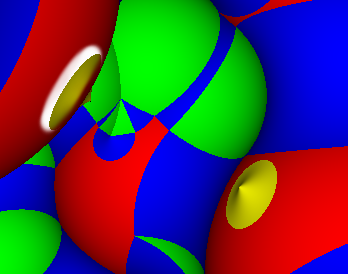
\includegraphics[height=1.4in]{image/isolated-cutaway2.png}
    %\caption{An \textit{isolated} torus.}
		\label{fig:isolated-cutaway}
  \end{subfigure}%
  \quad
  \begin{subfigure}[t]{0.4\columnwidth}
    \centering
    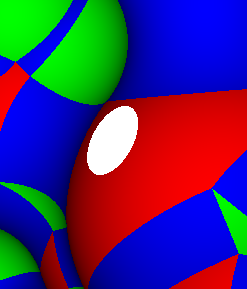
\includegraphics[height=1.4in]{image/isolated-hole.png}
    %\caption{A hole in a spherical patch.}
		\label{fig:isolated-hole}
  \end{subfigure}
\caption{Example of an isolated torus between two spheres.
	Left: Isolated tori do not have neighboring triangles, therefore the surface component to which they belong cannot be determined directly from the surface graph. 	Right: An isolated torus cuts circular holes into its neighboring spherical patches.}
\end{figure}

An \textit{isolated} torus can be encountered, while writing toroidal patches for ray-casting.
We add this torus into the buffer for ray-casting and we also mark it for later processing.
Later on, when the detection of surface components is done, we run another kernel which assigns the \textit{isolated} tori with their surface labels.
The assignment is done by inspecting neighboring spheres of the tori.
There can be two cases:
\begin{enumerate}
  \item One of the spheres forms only one patch. Then, the torus lies in the same surface component as this patch.
	\item Both spheres form two or more patches. We find a neighboring patch of the torus by employing the point in spherical patch test (see Section~\ref{sec:spherical-patches}). Then, the torus lies in the same surface component as its neighboring patch.
\end{enumerate}

The clipping of fragments in affected spherical patches can be done using a clipping plane or a visibility sphere of a torus.
We use the latter approach, since visibility spheres for tori were already computed in a previous phase of our technique.
Here, our kernel writes a texture, similarly to Krone et al.~\cite{krone2011parallel}, which stores for each sphere all visibility spheres that intersect it.
When ray-casting spherical patches, we use this texture to discard all fragments that are inside of an intersecting visibility sphere.
